\input{preamble}

\begin{document}


\noindent
Pokolorujmy ten prostokąt w szachownicę. Załóżmy, że lewe dolne pole będzie koloru czarnego. Skoro prostokąt $\mathcal{P}$ ma bok nieparzystej długości, to wszystkie jego narożne pola będą koloru czarnego. Również zawiera on o jedno pole czarne więcej niż zawiera pól białych. 

\vspace{10px}
\noindent
Każdy z prostokątów, na które jest on podzielony można zaklasyfikować do jednego z trzech typów:
\begin{itemize}
	\item Prostokąt, który ma dwa pola narożne białe i dwa pola narożne czarne. Zawiera on tyle samo pól białych, co czarnych;
	\item Prostokąt o czterech polach narożnych białch. Zawiera on o jedno pole białe więcej;
	\item Prostokąt o czterech polach narożnych czarnych. Zawiera on o jedno pole czarne więcej.
\end{itemize}

\begin{center}
	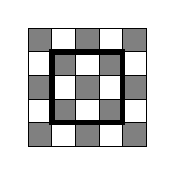
\begin{tikzpicture}[scale=0.3]

		\fill[color=gray] (0,0) rectangle (1,1);
		\fill[color=gray] (1,1) rectangle (2,2);
		\fill[color=gray] (2,2) rectangle (3,3);
		\fill[color=gray] (3,3) rectangle (4,4);
		\fill[color=gray] (4,4) rectangle (5,5);
		\fill[color=gray] (0,4) rectangle (1,5);
		\fill[color=gray] (0,2) rectangle (1,3);
		\fill[color=gray] (1,3) rectangle (2,4);
		\fill[color=gray] (2,4) rectangle (3,5);
		\fill[color=gray] (2,0) rectangle (3,1);
		\fill[color=gray] (3,1) rectangle (4,2);
		\fill[color=gray] (4,2) rectangle (5,3);
		\fill[color=gray] (4,0) rectangle (5,1);

		\draw (0,0) -- (5,0) -- (5,5) -- (0,5) -- cycle;
		\draw (0,1) -- (5,1);
		\draw (0,2) -- (5,2);
		\draw (0,3) -- (5,3);
		\draw (0,4) -- (5,4);


		\draw (1,0) -- (1,5);
		\draw (2,0) -- (2,5);
		\draw (3,0) -- (3,5);
		\draw (4,0) -- (4,5);

		\draw[line width=2pt] (1,1) rectangle (4,4);
		
	\end{tikzpicture}
\end{center}

\noindent
Skoro $\mathcal{P}$  zawiera o jedno pole czarne więcej, to pewien z rozpatrywanych prostokątów, nazwijmy go $P$ musi mieć czarne pola narożne. Zarówno $\mathcal{P}$, jak  $P$ mają czarne pola narożne, z czego łatwo wynika, że odległości między odpowiadającymi im bokami są tej samej parzystości.

\end{document}